\section{A benchmark problem with analytical solution}


Let $\Omega=[0,1]^3$, $\Lambda=\{x=\tfrac{1}{2}\}\times \{y=\tfrac{1}{2}\} \times [0,1] $
and $\Sigma=[\tfrac{1}{4}, \tfrac{3}{4}]\times [\tfrac{1}{4}, \tfrac{3}{4}]\times [0, 1]$.
Finally we let $\DD$ be the cross section of the virtual interface $\Gamma=\partial \Sigma$.
As a benchmark for the two formulations we consider the following coupled problems
%
\begin{subequations}\label{benchmark}
\begin{align}
\label{benchm_3d}
-\Delta u=f \quad &\text{in $\Omega$}\\
\label{benchm_1d}
-d_{zz}^2 \ud =g \quad &\text{on $\Lambda$}\\
u=u_b \quad &\text{on $\partial \Omega$},
\end{align}
\end{subequations}
where for formulation \eqref{eq:problem1} the mix-dimensional coupling constraint reads
\begin{equation}
  \label{eq:couple_1}
\trace{u} - \ext{\ud} = q_1\quad\text{ on }\Gamma,
\end{equation}
while for \eqref{eq:problem2} we set
\begin{equation}
    \label{eq:couple_2}
\avrc{u} - \ud = q_2\quad\text{ on }\Lambda.
\end{equation}
%
In \eqref{benchmark}-\eqref{eq:couple_2} the right-hand sides shall be defined as 
\begin{eqnarray*}
  &f=8\pi ^2 \sin (2\pi x) \sin (2\pi y),\quad &g={\pi ^2}\sin \left({\pi z}\right),\quad u_b=\sin (2\pi x) \sin (2\pi y),\\
  &q_1=\sin (2\pi x) \sin (2\pi y) - \sin \left({\pi z}\right),\quad &q_2=-\sin \left({\pi z}\right).
\end{eqnarray*}

The exact solution of \eqref{benchmark}, regardless of the coupling constraint,
is given by
%
\begin{eqnarray}
\label{benchm_sol3d}
u=\sin (2\pi x) \sin (2\pi y)\\
\label{benchm_sol1d}
%\ud=1+\exp(-z).
\ud=\sin \left({\pi z}\right).
\end{eqnarray}
%
Let us notice that $\ud$ satisfies homogeneous Dirichlet conditions at the boundary of $\Lambda$.
Moreover, the solution \eqref{benchm_sol3d}-\eqref{benchm_sol1d} satisfies on $\Gamma$ the relation
\begin{equation}\label{benchm_flux}
L=\nabla u \cdot \textbf{n}_{\oplus}=d_z \ud n_{\oplus,z}=0,
\end{equation}
with $n_{\oplus,z}$ the $z-$component of the normal unit vector to $\Gamma$.

We prove that \eqref{benchmark} is solution of \eqref{eq:problem2} in the
simplified case in which the starting 3D-3D problem is
\begin{subequations}\label{eq:dirneu_simple}
\begin{align}
- \Delta \up  &= f  && \text{ in } \Omega_{\oplus},\\
- \Delta \uf &= g  && \text{ in } \Sigma,\\
-\nabla \uf \cdot \nn_{\ominus} &= -\nabla \up \cdot \nn_{\ominus}  && \text{ on } \Gamma,\\
\uf - \up &= q_i  && \text{ on }  \Gamma,\\
\up &= h && \text{ on } \partial \Omega.
\end{align}
\end{subequations}
instead of \eqref{eq:dirneu}. Therefore the reduced problem in \eqref{eq:problem1} and
\eqref{eq:problem2} become respectively
%
\begin{subequations}\label{eq:problem1_simple}
\begin{align}
\label{eq:problem1_simple_eq1}
&(\nabla u,\nabla v)_{L^2(\Omega)} + |{\cal D}|(d_s \ud,d_s \vd)_{L^2(\Lambda)} 
+ \langle \trace{v}  - \ext{\vd}, \lambda \rangle_\Gamma
\\
\nonumber
&\qquad\qquad= (f,v)_{L^2(\Omega)} + |{\cal D}| (\avrd{g},\vd)_{L^2(\Lambda)}
\quad \forall v \in H^1_0(\Omega), \ \vd \in H^1_0(\Lambda)
\\
\label{eq:problem1_simple_eq2}
&   \langle \trace{u} - \ext{\ud} , \mu \rangle_\Gamma =  \langle q_1 , \mu \rangle_\Gamma
\quad \forall \mu \in H^{-\frac12}(\Gamma)\,.
\end{align}
\end{subequations}
and
\begin{subequations}\label{eq:problem2_simple}
  \begin{align}
    \label{eq:problem2_simple_eq1}
&(\nabla u,\nabla v)_{L^2(\Omega)} + |{\cal D}|(d_s \ud,d_s \vd)_{L^2(\Lambda)} 
+ |{\partial \cal D}| \langle \avrc{v} - \vd, \ld \rangle_{H^{-\frac12}(\Lambda)} 
\\
\nonumber
&\qquad\qquad= (f,v)_{L^2(\Omega)} + |{\cal D}| (\avrd{g}, \vd)_{L^2(\Lambda)}
\quad \forall v \in H^1_0(\Omega), \ \vd \in H^1_0(\Lambda)
\\
\label{eq:problem2_simple_eq2}
&  |\partial {\cal D}| \langle \avrc{u} -  \ud, \md \rangle_{H^{-\frac12}(\Lambda)} =
|\partial {\cal D}| \langle \avrc{q_2}, \md \rangle_{H^{-\frac12}(\Lambda)}
\quad \forall \md \in H^{-\frac12}(\Lambda)\,.
\end{align}
\end{subequations}

Let us prove that \eqref{benchm_sol3d}-\eqref{benchm_sol1d} is solution of
\eqref{eq:problem2_simple}. Using the integration by part formula and homogeneous
boundary conditions on $\Omega$ and $\Lambda$, from \eqref{eq:problem2_simple_eq1} we have
\begin{align*}
&-(\Delta u, v)_{L^2(\Omega)} - |{\cal D}|(d^2_{ss} \ud, \vd)_{L^2(\Lambda)} 
+ |{\cal D}|\langle \avrc{v}  - \vd, \ld \rangle_\Lambda
\\
\nonumber
&\qquad\qquad= (f,v)_{L^2(\Omega)} + |{\cal D}| (\avrd{g},\vd)_{L^2(\Lambda)}
\quad \forall v \in H^1_0(\Omega), \vd \in H^1(\Lambda).
\\
\end{align*}
Since $\ld=\avrc{L}=0$ and \eqref{benchm_sol3d} satisfies \eqref{benchm_3d} and \eqref{benchm_sol1d}
satisfies \eqref{benchm_1d}, we have that
\begin{align*}
-(\Delta u, v)_{L^2(\Omega)} =  (f,v)_{L^2(\Omega)} \\
-|{\partial \cal D}|(d^2_{ss} \ud, \vd)_{L^2(\Lambda)}  = |{\cal D}| (\avrd{g},\vd)_{L^2(\Lambda)},
\end{align*}
Thus \eqref{benchm_sol3d}-\eqref{benchm_sol1d} satisfy \eqref{eq:problem2_simple_eq1}.
The fact that the solution satisfy \eqref{eq:problem2_simple_eq2} follows from \eqref{eq:couple_2}.

We can prove in a similar way that \eqref{benchm_sol3d}-\eqref{benchm_sol1d}, with $\lambda=L=0$
satisfy \eqref{eq:problem1_simple}. Note in particular that $q_1$ is such that
$\trace{u} - \ext{\ud} = q_1$ on $\Gamma$.

\subsection{Numerical experiments. $\mathcal{T}^{\Omega}_h$ conforming to $\Gamma$}\label{sec:experiment_conform}
Using the benchmark problem \eqref{benchmark} we now investigate convergence
properties of the two formulations. To this end we consider a \emph{uniform} tessilation
of $\mathcal{T}^{\Omega}_h$ of $\Omega$ consisting of tetrahedra with diameter $h$.
Further, the discretization shall be geometrically \emph{conforming} to both $\Lambda$
and $\Gamma$ such that the tessilations $\mathcal{T}^{\Gamma}_h$, $\mathcal{T}^{\Lambda}_h$
are made up of facets and edges of $\mathcal{T}^{\Omega}_h$ respectively, cf. Figure \ref{fig:mesh}
for illustration.


\begin{table}
%%   %%%
\begin{minipage}[b]{0.35\linewidth}
 \centering
 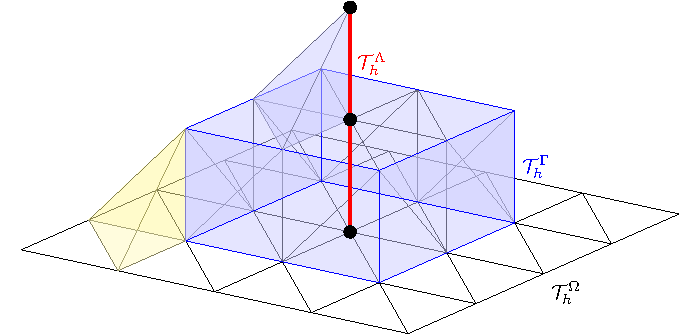
\includegraphics[width=\textwidth]{graphics/conform_mesh.pdf}
 \vspace{-20pt}
 \captionof{figure}{
$\Lambda$ and $\Gamma$ conforming discretization of $\Omega$
   used for \eqref{eq:problem1_simple} and \eqref{eq:problem2_simple}.   
 }
\label{fig:mesh}
\end{minipage}
\hspace{2pt}
\begin{minipage}[b]{0.63\textwidth}
  \scriptsize{
  \begin{center}
    \begin{tabular}{l|llll}
      \toprule
    $h^{-1}$ & $\norm{u-u_h}_{1, \Omega}$ & $\norm{\ud-\udh}_{1, \Lambda}$ & $\norm{\lambda-\lambda_h}_{-\tfrac{1}{2},\Gamma}$ & $\norm{\lambda-\lambda_h}_{0,\Gamma}$\\
      \hline
4  & 3.4E0(--)    & 5.3E-1(--)   & 2.9E0(--)    &8.7E0(--)    \\
8  & 1.7E0(0.99)  & 2.6E-1(1.06) & 6.1E-1(2.25) &1.9E0(2.21)  \\
16 & 8.7E-1(0.99) & 1.3E-1(1.02) & 1.4E-1(2.13) &4.7E-1(1.99) \\
32 & 4.4E-1(1.00) & 6.3E-2(1.00) & 3.4E-2(2.03) &1.3E-1(1.80) \\
64 & 2.2E-1(1.00) & 3.1E-2(1.00) & 8.6E-3(2.00) &4.2E-2(1.68) \\
\midrule
$h^{-1}$ & $\norm{u-u_h}_{1, \Omega}$ & $\norm{\ud-u_{\odot, h^{\prime}}}_{1, \Lambda}$ & $\norm{\ld-\ldh}_{-\tfrac{1}{2}, \Lambda}$ & $\norm{\ld-\ldh}_{0, \Lambda}$\\
\hline
4   & 3.1E0(--)    & 5.4E-1(--)   & 4.4E-2(--)   & 7.8E-2(--)  \\
8   & 1.7E0(0.87)  & 2.6E-1(1.06) & 1.1E-2(2.01) & 1.9E-2(2.01)\\
16  & 8.6E-1(0.96) & 1.3E-1(1.02) & 2.7E-3(2.01) & 4.8E-3(2.02)\\
32  & 4.4E-1(0.99) & 6.3E-2(1.00) & 6.7E-4(2.01) & 1.2E-3(2.01)\\
64  & 2.2E-1(1.00) & 3.1E-2(1.00) & 1.7E-4(2.01) & 3.0E-4(2.01)\\
128 & 1.1E-1(1.00) & 1.6E-2(1.00) & 4.1E-5(2.01) & 7.4E-5(2.00)\\
\bottomrule
  \end{tabular}
  \end{center}
  }
  \captionof{table}{Error convergence of \eqref{eq:problem1_simple} and \eqref{eq:problem2_simple}
    on a benchmark problem \eqref{benchmark}. Continuous linear Lagrange
    elements are used.
  }
  \label{tab:error_conform}
  \end{minipage}
\end{table}

Considering inf-sup stable discretization in terms of continuous linear Lagrange
($P_1$) elements (for all the spaces), Table \ref{tab:error_conform}
lists the errors of formulations \eqref{eq:problem1_simple} and \eqref{eq:problem2_simple}
on the benchmark problem. It can be seen the error in $u$ and $\ud$ in $H^1$ norm
converges linearly (as can be expected due to $P_1$ element discretization).
Moreover, the error of the Lagrange multiplier approximation in $H^{-1/2}$ norm
decreases quadratically. In the light of $P_1$ discretization this rate appears
superconvergent. We speculate that the result is due to the fact that the
exact solution is particularly simple, $\lambda=\ld=0$.
%In case of the results for
%\eqref{eq:problem1_simple} the rate can also be due to the fact that the
%error is interpolated into the same finite element space as the approximation $Q_h$.
We remark that for $u$ and $\ud$ the error is interpolated into the finite element space of
piecewise quadratic \emph{discontinous} functions. For \eqref{eq:problem2_simple} we
evaluate the fractional norm and interpolate the error using piecewise continuous
cubic functions. This is due to the fact that evaluating the fractional norm in higher order spaces
for on $\Gamma$ is prohibitively costly. For the sake of comparison with non-conforming formulation of \eqref{eq:problem2} from
\S\ref{sec:unfit2} Table \ref{tab:error_conform} also
lists the error of the Lagrange multiplier in the $L^2$ norm. Here, quadratic convergence is observed
for \eqref{eq:problem2_simple}. For \eqref{eq:problem1_simple} the rate between 1.5 and 2.

We plot the numerical solution of problem \eqref{eq:problem1_simple} and \eqref{eq:problem2_simple} in
Figure \ref{fig:sol_benchm1} and \ref{fig:sol_benchm2}, respectively.

\begin{figure}
\centering
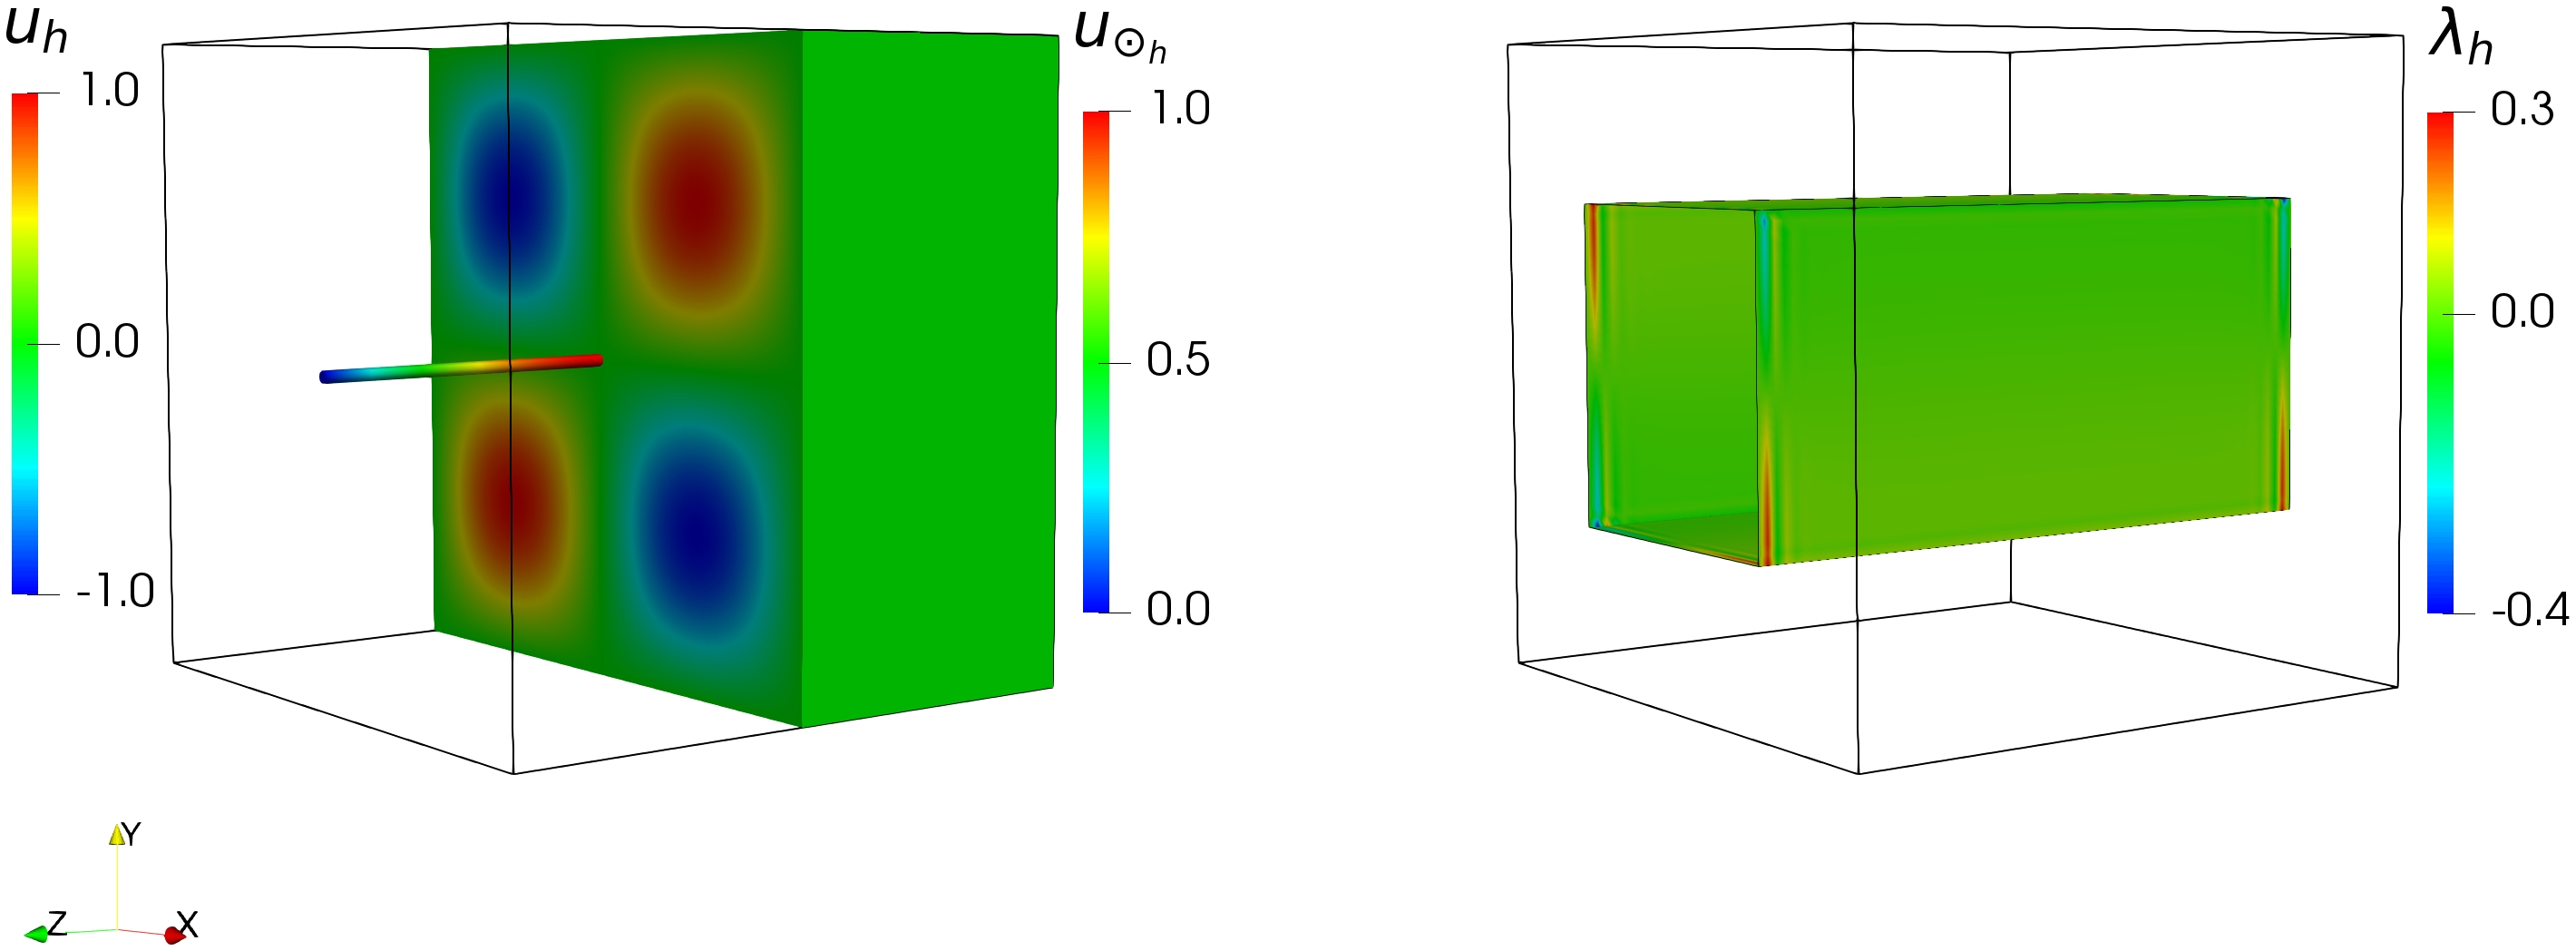
\includegraphics[width = 0.9\textwidth]{./graphics/mfs_LM2d}
\caption{Numerical solution of problem \eqref{eq:problem1_simple}: functions $u_h$ and $\udh$ on the left and the Lagrance multiplier $\lambda_h$ on the right.}\label{fig:sol_benchm1}
\end{figure}


\begin{figure}
\centering
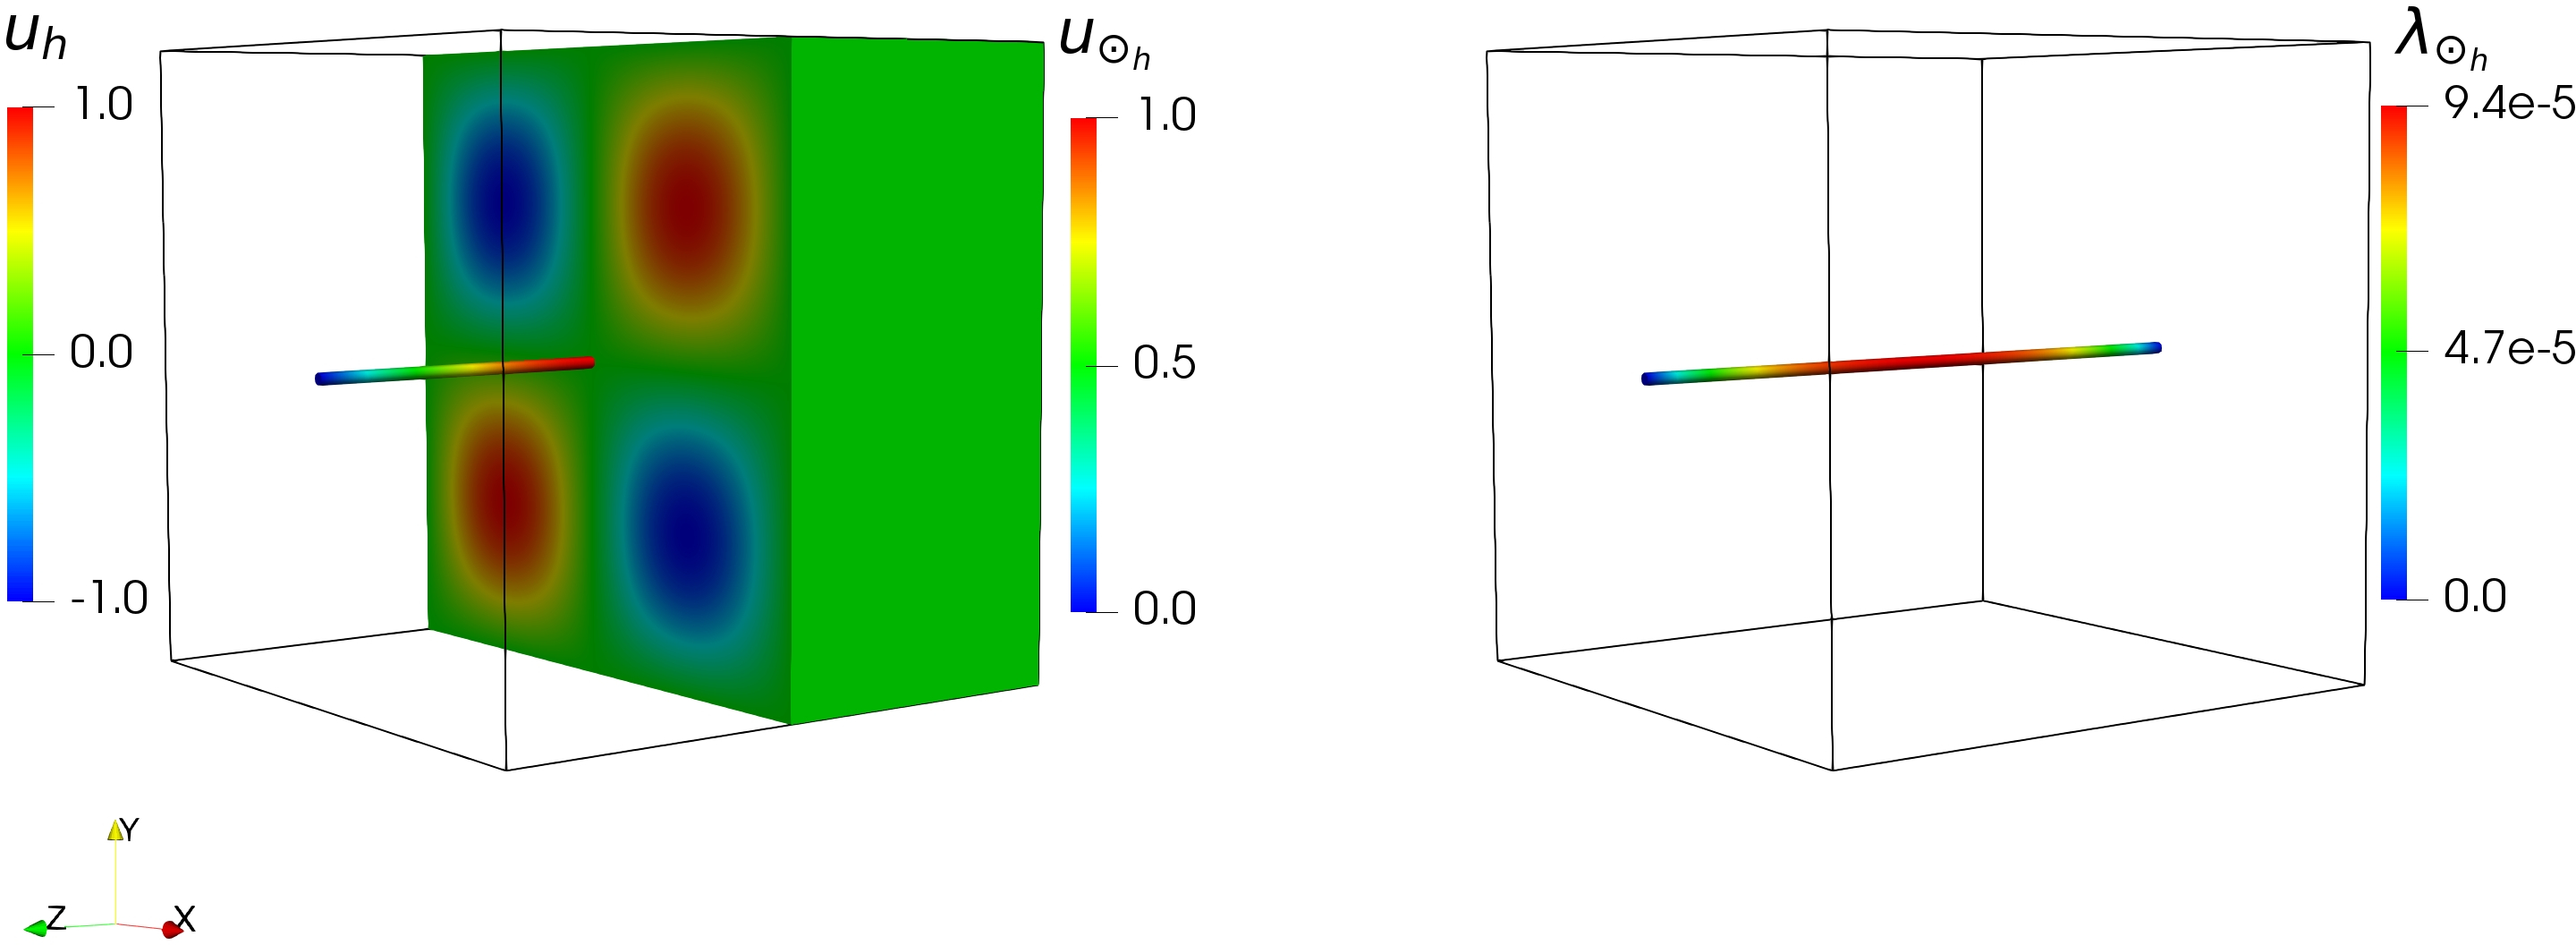
\includegraphics[width = 0.9\textwidth]{./graphics/mfs_LM1d}
\caption{Numerical solution of problem \eqref{eq:problem2_simple}: functions $u_h$ and $\udh$ on the left and the Lagrance multiplier ${\ld}_h$ on the right.}\label{fig:sol_benchm2}
\end{figure}


\subsection{Numerical experiments. $\mathcal{T}^{\Omega}_h$ non-conforming to $\Gamma$}\label{sec:experiment_nonconform}
Using benchmark problem \eqref{benchmark} we consider \eqref{eq:problem2} in the
setting of \S \ref{sec:unfit2}. To this end we let $\mathcal{T}^{\Omega}_h$ be a uniform
tessilation of $\Omega$ such that no cell $\mathcal{T}^{\Omega}_h$ has any edge
lying on $\Lambda$. Further we let $h^{\prime}=h/3$ in $\mathcal{T}^{\Lambda}_{h^{\prime}}$,
cf. Figure \ref{fig:unfit}.

Using discretization in terms of $P_1$-$P_1$-$P_0$ element Table \ref{tab:error_unfit}
lists the error of the stabilized formulation of \eqref{eq:problem2}. A linear
convergence in the $H^1$ norm can be observed in the error of $u$ and $\ud$. We
remark that the norms were computed as in \S\ref{sec:experiment_conform}. For simplicity
the convergence of the multiplier is measured in the $L^2$ norm rather then the $H^{-1/2}(\Gamma)$
norm used in the analysis. Then, convergence exceeding order 1.5 can be observed, however,
the rates are rather unstable.

\miro{The solution is plotted in ..... I guess there should be some zoom in on the
cut cells.}

\begin{table}
%%   %%%
\begin{minipage}[b]{0.35\linewidth}
 \centering
 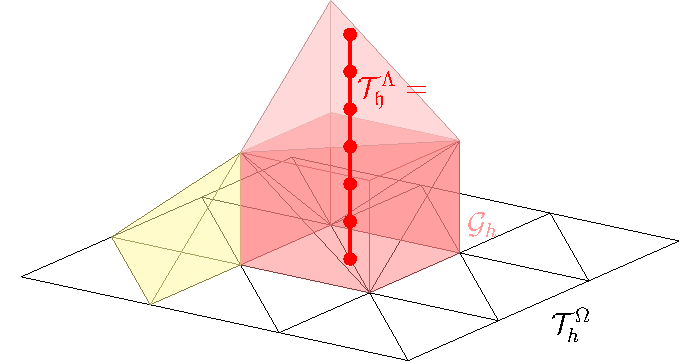
\includegraphics[width=\textwidth]{graphics/nonconform_mesh.pdf}
 \vspace{-20pt}
 \captionof{figure}{
   Sample discretization of the benchmark geometry in the non-conforming case. 
 }
\label{fig:unfit}
\end{minipage}
\hspace{2pt}
%%%
    \begin{minipage}[b]{0.62\linewidth}
      %%%
  \scriptsize{
  \begin{center}
    \begin{tabular}{l|lll}
      \toprule
    $h^{-1}$ & $\norm{u-u_h}_{1, \Omega}$ & $\norm{\ud-\udh}_{1, \Lambda}$ & $\norm{\ld-\ldh}_{0,\Lambda}$\\
      \hline
5   & 2.6E0(--)    & 2.3E-1(--)   & 1.7E-1(--) \\ 
9   & 1.5E0(0.84)  & 9.4E-2(1.42) & 7.1E-2(1.36)\\
17  & 8.1E-1(0.94) & 4.3E-2(1.18) & 2.9E-2(1.37)\\
33  & 4.2E-1(0.98) & 2.1E-2(1.06) & 7.9E-3(1.91)\\
65  & 2.1E-1(0.99) & 1.1E-2(1.02) & 2.6E-3(1.64)\\
129 & 1.1E-1(1.00) & 5.2E-3(1.01) & 8.5E-4(1.61)\\
\bottomrule
    \end{tabular}
  \end{center}    
}    
  \captionof{table}{
    Error convergence of \eqref{eq:problem2_simple} on a benchmark problem \eqref{benchmark} in case
    $\mathcal{T}^{\Omega}_h$ does not conform to $\Lambda$.}
  \label{tab:error_unfit}    
  \end{minipage}
\end{table}

\subsection{Comparison}
In Tables \ref{tab:error_conform}, \ref{tab:error_unfit} one can observe that 
all the formulations yield practically identically accurate approximations of $u$.
Futher, compared to the conforming case, the stabilized formulation \eqref{eq:problem2}
results in a greater accuracy of $u_{\cdot, h}$ as the underlying mesh $\mathcal{T}^{\Lambda}_{h}$ is
here finer. Due to the different definitions in the three formulations, comparision of the Lagrange
multiplier convergence is not straightforward. We therefore limit ourselves to a
comment that in the $L^2$ norm all the formulations yield faster than linear convergence.

In order to discuss solution cost of the formulations we consider 
the resulting preconditioned linear systems. In particular, we shall compare
spectral condition numbers and the time to convergence of the preconditioned
minimal residual (MinRes) solver with the with stopping criterion requiring
the relative preconditioned residual norm to be less than $10^{-8}$. We remark
that we shall ignore the setup cost of the preconditioner.

Following operator preconditioning technique \cite{mardal2011preconditioning} we
propose as preconditioners for \eqref{eq:problem1} and \eqref{eq:problem2} in the
conforming case the (approximate) Riesz mapping with respect to the inner products of
the spaces in which the two formulations were proved to be well posed.
In particular, the preconditioner for the Lagrange multiplier relies on
(the inverse of) the fractional Laplacian $-\Delta^{-1/2}$ on $\Gamma$ for
\eqref{eq:problem1_simple} and $\Lambda$ for \eqref{eq:problem2_simple}.
A detailed analysis of the preconditioners will be presented in a separate
work. We remark that in both cases the fractional Laplacian was here realized
by spectral decomposition \cite{kuchta2016preconditioners}.

For the unfitted stabilized \eqref{eq:problem2} the Lagrange multiplier preconditioner
uses a Riesz map with respect to the inner product due to $L^2(\mathcal{G}_h)$ and
the stabilization \eqref{eq:stab}, i.e.
\[
({\ld}_h, {\md}_h) \mapsto \sum _{K\in \mathcal{G}_h}\int_{K}{\ld}_h {\md}_h + \sum _{K\in \mathcal{G}_h} \int_{\partial K \setminus \partial \mathcal{G}_h} h \llbracket {\ld}_h \rrbracket \llbracket {\md}_h \rrbracket.
\]
This simple choice does not yield bounded
iterations. However, establishing a robust precondtioner in this case 
is beyond the scope of the paper and shall be pursued in the future works.


In Table \ref{tab:cost} we compare solution time, number of iterations and
condition numbers of the (linear systems due to the) three formulations.
Let us first note that the proposed preconditioners for \eqref{eq:problem1} and
\eqref{eq:problem2} in the conforming case seem robust with respect to discretization
parameter as the iteration counts and condition numbers are bounded in $h$.
We then see that the solution time for \eqref{eq:problem1_simple} is about 2 times
longer compared to \eqref{eq:problem2_simple} which is about 4 times more expensive
than the solution of the Poisson problem \eqref{benchm_3d}. This is in addition to the
higher setup costs of the preconditioner which in our implementation involve solving
an eigenvalue problem for the fractional Laplacian. Therefore it is advantageous to keep
the multiplier space as small as possible. We remark that the missing
results for \eqref{eq:problem1_simple} in Table \ref{tab:cost} and \ref{tab:error_conform}
are due to the memory limitations which we encounter when solving the eigenvalue problem
for the Laplacian, which for finest mesh involves cca 32 thousand eigenvalues, cf. Appendix \ref{sec:appendix}.
%

Due to the missing proper preconditioner for the Lagrange multiplier block the
number of iterations in the third, unfitted formulation can be seen to approximatly
double on refinement. 

\begin{table}
  \scriptsize{
  \begin{center}
    \begin{tabular}{l|lll|lll|lll|ll}
      \toprule
      \multirow{2}{*}{$l$} & \multicolumn{3}{c|}{\eqref{eq:problem1}} & \multicolumn{3}{c|}{\eqref{eq:problem2}} & \multicolumn{3}{c|}{ Stabilized \eqref{eq:problem2}} & \multicolumn{2}{c}{\eqref{benchm_3d}}\\
      \cline{2-12}
      & \# & $T\left[s\right]$ & $\kappa$ & \# & $T\left[s\right]$ & $\kappa$ & \# & $T\left[s\right]$ & $\kappa$ & \# & $T\left[s\right]$\\
      \hline
      1 & 20 & 0.03  & 15.56 & 9  & 0.02  & 3.04 & 21  & 0.01   & 9.70  &3 & $<0.01$\\ 
      2 & 35 & 0.06  & 16.28 & 17 & 0.03  & 4.67 & 31  & 0.03   & 15.87 &4 & $<0.01$\\ 
      3 & 38 & 0.14  & 16.64 & 22 & 0.06  & 6.25 & 53  & 0.15   & 32.93 &5 & 0.01   \\ 
      4 & 39 & 1.70  & 16.75 & 24 & 0.89  & 7.03 & 110 & 4.54   & 61.48 &5 & 0.12   \\ 
      5 & 38 & 12.04 & 16.78 & 20 & 5.21  & 5.02 & 232 & 59.43  & 94.25 &5 & 0.90  \\ 
      6 & -- & --    & --    & 17 & 28.77 & --   & 507 & 832.90 & --    &6 & 7.75  \\ 
      \bottomrule
    \end{tabular}
    \end{center}
    }
  \caption{Cost comparison of the formulations across refinement levels $l$.
    Number of MinRes iterations and the conditioned number of the preconditioned
    problem is denoted by $\#$ and $\kappa$ respectively. Time till convergence
    of the iterative solver (excluding the setup) is shown as $T$. Results of algebraic
    multigrid preconditioned conjugate gradient method for 3D Poisson are shown
    in the last 2 columns.
  }
\label{tab:cost}
\end{table}








%\begin{remark}
%Let us notice that the 3D solution \eqref{benchm_sol3d} is such that $\avrc{u}=0$. Therefore in \eqref{benchmark} it is like we are solving two separated problems, one in $\Omega$ and the other on $\Lambda$.
%\end{remark}
%\begin{remark}
%It would be interesting to make a comparison between the solution of the fully coupled 3D-3D problem \eqref{eq:dirneu} (also in the simplified case of type \eqref{eq:dirneu_simple}) and the solution of the reduced problems \eqref{eq:problem1} and \eqref{eq:problem2}. 
%Therefore, we could set the values of the data of the problem such that the reduced formulation becomes non-trivial and fully coupled.
%Then, we will solve both the original and reduced problem to observe the differences in the solutions and the values of the Lagrange multiplier.
%\end{remark}
